Our objective is to analyze multiple projects, checking whether we can build  or not every snapshot.
For those snapshots whose build fails, we study the build logs to determine which are the most common errors that prevent a snapshot from being buildable, grouping and categorizing errors in a taxonomy.

%Reproducibility is a topic of interest among researchers to validate other publications~\cite{RODRIGUEZPEREZ2018164} and projects~\cite{4693714} through reproducibility, in addition to offering solutions that facilitate reproducibility in the future~\cite{DBLP:journals/corr/Weber17,DockerReproducibility2016,Boettiger:2015:IDR:2723872.2723882}. For this reason,
 
We have tried to make our experiment reproducible so that any researcher can obtain the same results as we do or use our data for other investigations.
The reproducibility package for this work can be found in a public repository\footnote{\url{https://github.com/Maes95/TFM-Buildability/tree/ReproducePackage/Tools}}.

%\mica{New section to discuss reproducibility of the project?}
%\grex{This belongs to the methodology section and should be better a footnote with the URL, not a cite.}

\section{Subject programs}

To choose what projects are suitable for this study, we consider some desirable characteristics that make them easy to build:

\begin{itemize}
	\item Using a compiled language (e.g., Java or C++), so that when developing, type-safety is enforced during the build phase, avoiding type problems in runtime.
In addition, we can obtain more information at the build phase than from projects using a dynamic language.
	\item Project dependencies are simple to obtain, for example, from a remote repository.
	\item The environment in which the project was built is easy to set up, or has no impact on the build.
\end{itemize}

Following Easterbrook \emph{et al.}~\cite{easterbrook2008selecting}, we selected six exploratory case studies to gain a deep understanding of the buildability in six open source projects.
For this purpose, we selected projects written in Java, a static typed programming language that is platform-independent, with a freely available compiler.
Java has also backward compatibility and multiple tools to manage dependencies like Maven, Gradle or Ant.
In order to study the buildability of a project, the history of the projects needs to be available through some source control management (SCM) system.
The selected projects are available in Git repositories, so we used Git to traverse their history.

Table~\ref{table:projects} shows the six open source Java projects selected for the study.
For each project, we display the number of snapshots (commits) that are available in their respective git repositories, and the build system used by the project to compile the source code and generate the binaries.
Five projects come from a common dataset in software research, Defects4J~\cite{Just:2014:DDE:2610384.2628055}.
These projects are commonly used for research in Software Testing.
It is important to note that they are small projects with a limited set of dependencies.
The only exception is the Closure project, with 12 dependencies, which are included in the source code without the need to recover them from an external repository.

%\grex{Could we have the number of dependencies as well? As I suppose they vary over time, it would be good to provide a range of the number of dependencies.}
To expand our dataset, we also analyze the Spring Framework project.
This project is a large multi-module project, widely used in the industry for developing Java web applications.
The complexity of this project is far beyond that of the Defects4J projects.
It has as well a higher number of dependencies.

\begin{savenotes}
	\begin{table}
		\caption{Projects used in this work}
		\label{table:projects}
		\centering
		\begin{tabular}{crcr}
			\toprule
			\bf{Project} & \bf{\# Snapshots} & \bf{{Build system}} & \bf{\# Dependencies}\\ 
			\midrule
			Closure Compiler & 2,858 & Ant & 12\footnote{Dependencies are in source files}\\
			Commons-lang & 3,570 & Maven & 3\\
			Commons-math & 4,878 & Maven & 1\\
			Mockito & 2,639 & Gradle & 4\\
			Joda-Time & 1,717 & Maven & 2\\
			Spring Framework & 17,382 & Gradle & 20\footnote{Optional dependencies are not counted}\\
			\bottomrule
		\end{tabular}
	
	\end{table}
\end{savenotes}

\section{Analysis process}

The analysis consisted in two phases, a first one for checking buildability of the project (\textit{Check build process}), and a second one for analyzing the data collected of the failed builds (\textit{Log analysis}) in order to perform the classification.

%\grex{I don't know if ``experiment'' is the right wording}

\subsection{Check build process}

This process is shown in Figure~\ref{fig:commitHist}.
It starts with the most recent commit of the project.
This commit is checked out, and the project is built from its source files using the appropriate build system for the project (as defined in Table~\ref{table:projects}).
To determine the build status, we check the exit code of the build process: zero signifies success, and non-zero signifies failure.
If the build succeeds, it is marked as success.
Otherwise, it is marked as failure and the logs generated during the build process are saved for later inspection.
Then we go back to the previous commit, and repeat the whole process.
This process is repeated until we reach the first commit in the repository.
Figure~\ref{fig:commitHist} summarizes the process in a visual form.

% \begin{figure}[h]
% 	\centering    
% 	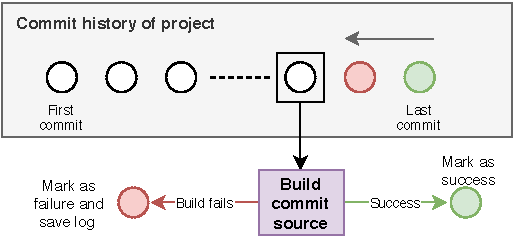
\includegraphics[width=12cm]{img/CommitHist.pdf}
% 	\caption{Check build process}
% 	\label{fig:commitHist}
% \end{figure}

Due to the large number of commits in the history of the selected projects, building them manually is not practical.
In order to automate the process, we developed a Python script that given a configuration file, a build script and the git project, basically executes the process described above iteratively for each commit.
To build each project, the basic commands of each construction tool have been used, taking into account the documentation of each project (e.g., a Maven build is shown in Listing~\ref{listing:mvnscrpt}).
In most projects, it is important to clean the output folders to avoid reusing files when changing between commits.
To reproduce these steps in a simple way without having to worry about the environment or the necessary technologies, this execution is encapsulated in a Docker\footnote{https://www.docker.com} container.

%\mica{Ampliar esto mencionando que incluye este paquete}

%\grex{I would like to hear something about the dependencies here...I remember hearing from Michel that he set up an environment where he run the experiment... please, include that info here!}

\begin{lstlisting}[caption={Example of a Maven build command},captionpos=b, label={listing:mvnscrpt}]
                      mvn clean install -Dmaven.test.skip=true
\end{lstlisting}


\subsection{Log analysis} 
\label{sssec:logAnalysis}

Our analysis (depicted in Figure~\ref{fig:AnalysisProcess}) takes as input:
   i) the commit history of the project (where each commit is marked as success or failure), and
   ii) the logs for the commits marked as a failure.
Our aim is to perform an analysis of the logs to determine the reasons why the build failed.

% \begin{figure}[h]
% 	\centering    
% 	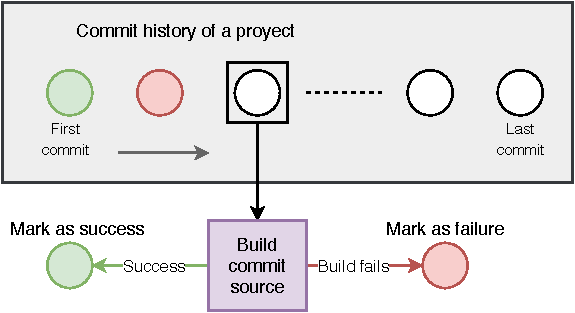
\includegraphics[width=12cm]{img/AnalysisProcess.pdf}
% 	\caption{Analysis process for builds that fail.}
% 	\label{fig:AnalysisProcess}
% \end{figure}

We assume that consecutive commits which fail between two successful commits are likely to contain the same error.
Based on this idea, choosing a log from a group of consecutive commits, we can extract the error trace that identifies the problem and generate a pattern from it.
Once we have a consistent number of patterns, we apply them in order (from more specific to more generic) to each log, stopping when a match occurs, continuing with the next log.
This process is iterative: new patterns are generated to eliminate very generic patterns and group the logs better.
We finish the process when all logs match a pattern and can be grouped without confusion.

We will call this error trace a \textbf{symptom}.
We then group similar patterns together, in order to identify those logs that share the same symptom.
For each symptom that we find, a \textbf{cause} (i.e., the error that causes the symptom) can potentially be attributed to it.
The cause, in many cases and due to the Java logging system, can be extracted together with the symptom.
In other cases, the cause is more ambiguous and requires interpreting the log along with the failed version of the project, exploring it in detail (sometimes at a very low-level).
In a next step, our intention is to categorize the error according to its nature using a method for taxonomy development.

%Once the cause is determined, we assess \textbf{if the error could be solved} by applying a change -- or if it is unsolvable.
%In case it is solvable, it is necessary to determine if it needs a) a simple change (e.g., adding a trivial script during the build) or b) a major change is necessary (e.g., a non-trivial modification of the source code).
%\michel{We should mantain this? We have no solutions for the errors}

To clarify the process, we present a didactic example is shown in Listing~\ref{listing:pattern}.
In this case, an error pattern is applied to the log obtained after a failed execution in the Spring Framework.

% \textcolor{black}{Pattern: }
\begin{center}
	\begin{lstlisting}[linewidth=\linewidth, caption={SpringFramework Log - Commit 8961}, captionpos=b, label={listing:pattern}]
	<@\textbf{Pattern: }@><@\textbf{\textcolor{violet}{Could not find (.+)}}@>
	<@\textbf{Log with pattern matching: }@>
	FAILURE: Build failed with an exception.
	
	* What went wrong:
	Could not resolve all dependencies for configuration ':spring-messaging:optional'.
	> <@\textbf{\textcolor{violet}{Could not find org.projectreactor:reactor-net:1.1.0.BUILD-SNAPSHOT.}}@>
	Required by:
	org.springframework:spring-messaging:4.1.0.BUILD-SNAPSHOT
	\end{lstlisting}
\end{center}


\begin{itemize}
	\item \textbf{{Symptom}}: The trace highlighted in the log can not resolve a dependency.
	\item \textbf{{Cause}}: An unspecified development (BUILD-SNAPSHOT) version is used and can not be recovered.
	%\item \textbf{{Could be solved?}}: It is resolvable, apparently easy, replacing the version with a stable one (release)
\end{itemize}



%\grex{I think it would be very didactic to show an example of an error log, to highlight where we see that we can find the cause. Doing this with an example, including a code excerpt would make the methodology easier to follow.}

Most of this process is automated.
We use Jupyter notebooks to make the interaction with the data more versatile.
We define the patterns by means of regular expressions (see Table~\ref{table:commmonErrors} for some examples).
Then, we count the number of occurrences of each pattern in the history of builds for the six projects under study.

\begin{table}
	\caption{Some common error patterns for Java projects}
	\label{table:commmonErrors}
	\begin{center}
		\begin{tabular}{c}
			\toprule
			\verb|error: (.+)\n(.+)| \\
			\midrule
			\verb=(> Could not resolve|> Could not find) (.+)= \\
			\midrule
			\verb|unable to resolve class (.+)| \\
			\midrule
			\verb|Exception in thread (.+)| \\
			\bottomrule
		\end{tabular}
	\end{center}
\end{table}

\section{Taxonomy development}\label{subsec:taxonomy}

The development of taxonomies is not limited only to software engineering, it has its origin in other fields such as biology~\cite{eldredge1980phylogenetic,sneath1973numerical} or Social Sciences~\cite{bailey1994typologies}.
The development of a taxonomy is not an easy task and requires to search a method that allows us to rigorously address the problem.
For the development of our taxonomy, we base ourselves on the well-known work by Nickerson, Varshney and Muntermann from the field of Information Systems~\cite{Nickerson2013}.
They propose a method to approach the creation of a taxonomy, which has been widely used by other researchers, e.g.~\cite{Krug2012APT,Geiger2011ManagingTC}.
The method is based on the fact that a taxonomy is a set of dimensions, each consisting of mutually exclusive and collectively exhaustive characteristics.
Therefore, each object that we want to classify will take a characteristic in each dimension.
The method allows us to combine both empirical-to-deductive and deductive-to-empirical approaches to identify the dimensions and corresponding characteristics.

In our case, the objects to be classified to obtain the taxonomy will be the causes, using the symptoms to classify them.
The classification will be done iteratively, using in each iteration a portion of the sample of symptoms obtained.
The ending condition will be that all the symptoms obtained have been classified, in addition to the objective ending conditions that the method defines.



